\chapter{Introduction}\label{chap:intro}

% \begin{quote}
% \normalsize\itshape
% \begin{flushright}
% \foreignlanguage{russian}{А вопросы… Вопросы не знают ответа —}\\
% \foreignlanguage{russian}{Налетят, разожгут и умчатся, как корь.} \\
% \foreignlanguage{russian}{Саша Черный} \\ \vskip 10pt
%  And the questions...  The questions lack answers, still missing:\\
%  They'll come and they'll burn, fade like measles, unkind.\\
%  Sasha Chorny
% \end{flushright}
% \end{quote}


%%%%%%%%%%%%%%%%%%%%%%%%%%%%%%%%%5
% Gneral Introduction, some talkson how deep generative mdoels are cool goes here
%%%%%%%%%%%%%%%%%%%%%%%%%%%%%%%%%5
In recent years, deep learning has seen significant advances, particularly in the field of generative models. Two of the most successful applications of Deep Generative Models (DGMs) are natural language processing and computer vision. In natural language processing, Large Language Models (LLMs), which usually constitute autoregressive generative models~\citep{graves2013generating} with a transformer-based architecture~\citep{vaswani2017attention}, have demonstrated impressive text generation capabilities~\citep{brown2020language,chowdhery2023palm}. They are capable of producing long and coherent texts across various contexts and have gained popularity in the form of chat bots~\citep{achiam2023gpt}. In computer vision, diffusion models are achieving impressive results in generating photorealistic images~\citep{dhariwal2021diffusion} and videos~\citep{ho2022video}.

% Bayesian inference and human learning \cite{xu2007word}

Practically, modeling the probability distribution of the data offers two main functionalities to the underlying model: sampling and likelihood estimates. A lot of attention is paid to the sampling functionality, as it can be used to produce completely novel datapoints, e.g. images that look like real ones but that were not observed by the model during training. Furthermore, conditional sampling from the distribution can be used to provide forecast or prediction in the situation when only part of the variables is observed. Access to the likelihood, if present, might also offer many benefits. This includes, but is not limited to, the estimation of uncertainty and the detection of out-of-distribution \cite{havtorn2021hierarchical, kadavath2022language}, as well as handling the missing data \cite{mattei2019miwae} and anomalies \citep{an2015variational}.

Latent Variable Models (LVMs) is a specific type of generative models, where the expressivity of the model is increased by introducing hidden (latent) variables.
These auxiliary random variables are meant to capture the underlying structure or factors that are not directly observed in the data, but influence the data generation process.
\marginnote[0.1\baselineskip]{Generative process defined by the latent variable model. First, latent variable $\rvz$ is sampled from the prior, then observed data point $\rvx$ is generated for a given latent.}
\begin{equation}
\begin{aligned}
    \rvz &\sim p(\rvz),\\
    \rvx &\sim p(\rvx|\rvz).
    \end{aligned}
\end{equation}
In Figure~\ref{fig:lvm_visualization} we schematically depict the latent space on the left and a mapping to the data space (dashed lines).
During training, Latent Variable Models are fitting the density to the observed datapoints to learn the unknown model parameters.
In this way, the trained generative model can produce realistic data samples and likelihood estimation.
Furthermore, these models approximate the conditional distribution of the unobserved latent variables given the data, enabling additional functionality of representation learning. 

\begin{figure}[t]
    \centering
\begin{tikzpicture}
    % Latent space (Left side)
    \node[align=center] at (-5.5,1) {\normalsize\textcolor{RedOrange}{$p(\rvz)$}};
        
    \shadedraw[shading=ball,  color=RoyalBlue!15, opacity=0.5]
    (-3,-.5)  .. controls (-3.5,-.5) and (-4,.5) .. 
    (-4.5,.5) .. controls (-5,.5) and (-6,0) .. 
    (-6,.5)   .. controls (-6,-1) and (-5,-1.5) .. 
    (-4.5,-1.5) .. controls (-4,-1.5) and (-3.5, -.5) .. (-3,-.5);
    
    % Contours in latent space
    \draw[RedOrange, thick, rotate=10] (-5,0.75) ellipse (0.4 and 0.2);
    \draw[RedOrange, thick] (-4,-0.5) ellipse (0.25 and 0.25);
    \draw[RedOrange, thick,rotate=10] (-4.75,0) ellipse (0.1 and 0.4);

    % Points in latent space
    \fill[RedOrange] (-5,-0.15) circle (2pt);
    \fill[RedOrange] (-4,-0.5) circle (2pt);
    \fill[RedOrange] (-4.65,-0.83) circle (2pt);

    % Data space (Right side)
    \node[align=center] at (-1,2) {\normalsize\textcolor{RoyalBlue}{$p(\rvx|\rvz)$}};

    % Axes in data space
    % \draw[thick, ->] (2,-1) -- (4,-1);
    % \draw[thick, ->] (3,-2) -- (3,2);

    % Image positions
    % \node at (1.1,1.5) {$\rvx_2$}; 
    \node at (1.3,1.5)  { 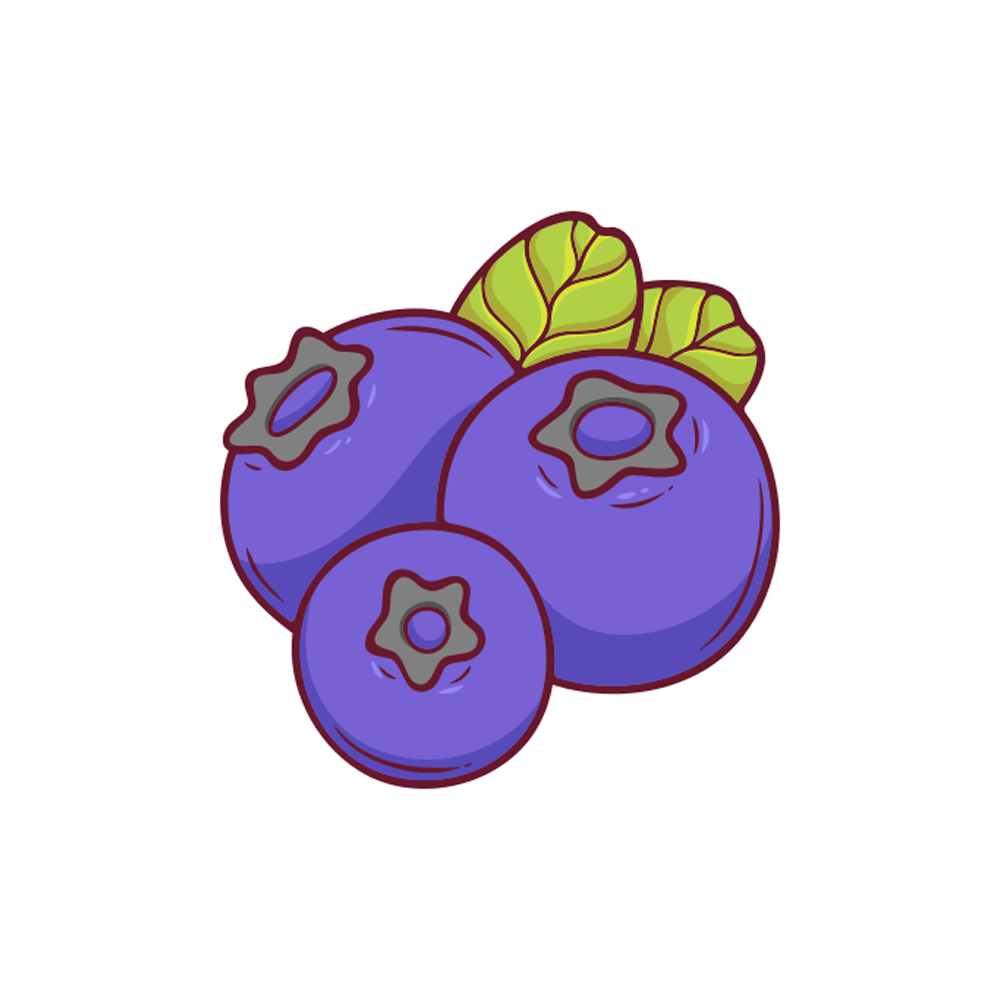
\includegraphics[width=1cm]{pics/0_intro/blueberry.png} }; 
    \node at (2.3,-0.5) { 
\includegraphics[width=1cm]{pics/0_intro/apple.png} }; 
    \node at (.9,-1.5) { 
\includegraphics[width=1cm]{pics/0_intro/banana.png} }; 
    % Dashed arrows from latent space to data space
    \draw[RoyalBlue, ->,dashed, thick] (-5,-0.15) to[out=20,in=160] (1,1.5);
    \draw[RoyalBlue, ->,dashed, thick] (-4,-0.5) to[out=30,in=150] (2,-0.5);
    \draw[RoyalBlue, ->, dashed, thick] (-4.65,-0.83) to[out=10,in=170] (.5,-1.5);

\end{tikzpicture}
    \caption{Latent Variable Models learn the mapping from the latent space (left) to the data space (right).}
    \label{fig:lvm_visualization}
\end{figure}
This thesis focuses on two latent variable models: Variational Autoencoder and Diffusion Models. These are the two most popular examples of LVMs. Both models parametrize probabilistic models with neural networks and are capable of producing extremely realistic data samples. 
% use neural network parametrized generative process to produce realistic data sample from the latent variables. 
These models differ in the way latent variable inference is defined. 
VAEs offer a more flexible approach of an encoder parametrized by a neural network. 
This encoder is trained to approximate a posterior distribution of the latent variable for a given data point.
Diffusion models, on the other hand, consider a non-trainable mapping from the input to the latent space. This mapping gradually adds Gaussian noise to the data, destroying the original signal. This limits the representation learning functionality of the model but improves the model scalability and training stability. 


\section{Research Goal}
Despite enormous successes, many challenges remain in the field of deep generative modeling~\citep{manduchi2024challenges} with latent variable models not being an exception. 
Identifying and addressing these challenges is an overarching research goal of this thesis.

\begin{quote}
\normalsize\itshape \noindent 
Identify and address weaknesses of latent variable generative models.
\marginnote[-0.1\baselineskip]{\itshape Research Goal}
\end{quote}

We focus on density estimation and representation learning as two general directions in which LVMs can be improved. 
 In the former aspect, our aim is to improve the likelihood estimation in various training scenarios or for a specific generative model. In the latter case, we focus on studying and improving the latent representations learned by the model. 

\subsection{Density estimation}
The first direction of research concerns the choice of the probabilistic model that improves the density estimation performance of the model. 
In Chapter~\ref{chap:boovae} we consider a dynamic continual learning scenario for a standard VAE model. This challenging training setup requires a model to learn a sequence of tasks while only observing one task at a time. It is important to dynamically increase the model capacity to learn new tasks and ensure that the model does not decrease it's performance on previously learned tasks.

Next, in Chapter~\ref{chap:dvp}, we propose a scalable optimal prior approximation for a deep hierarchical VAE. Learning an optimal prior approximation was previously shown to improve the density estimation of the VAE. However, it scales poorly when larger input and model size are considered. 

Further, in Chapter~\ref{chap:daed}, we focus on another LVM type, a diffusion model. We test the hypothesis that it is beneficial for model performance to decouple two functions of the generative process: adding useful information (generation) and removing uninformative bits (denoising). 

\subsection{Representation Learning}
The second research direction focuses on the properties of the latent representations learned by the models.
This is especially important for the downstream applications of the latent variable generative models. 

In Chapter~\ref{chap:adv_att} we test the robustness of latent representations to adversarial attacks. Adversarial attacks are small perturbations added to the input, which result in unexpected model behavior. Adversarily robust latent representations are crucial for a reliable and predictable performance of any downstream application of the model. 

Finally, In Chapter~\ref{chap:eqvae} we focus on the latent representation that preserves symmetry. Symmetries presented in the data are not guaranteed to be transferred to the latent space of the generative model. This can deteriorate the performance of downstream tasks where these symmetries are playing an important role. It is thus important to have the tools to formulate the latent variable generative model, which ensures that the mapping from the data space to the latent space is equivariant. 

\section{Dissertation Structure}
We provide an extensive background on Deep Generative Modeling in general and latent variable models specifically in Chapter \ref{ch:background}. We focus on the concepts and techniques used throughout the thesis and use this detailed context to formulate research questions addressed in each of the consecutive chapters. 

In the following, each chapter is based on one or more published papers. In total, the thesis is based on four $A^*$ conference publications, one journal article, and one workshop article.  
We divide them into two parts. Part~\ref{part:1} focuses on improved density estimation, and Part~\ref{part:2} takes a closer look at the properties of the learned data representations. 

We have chosen to keep the papers consistent with the original publication, which allows reading each chapter as an independent unit. 
Each paper is accompanied by an appendix which is located at the end of the dissertation.
In Table \ref{tab:papers_and_contributions} we arrange the articles according to the topic, so that the reader interested in a particular aspect can refer to the corresponding chapter.

\begin{table}[!ht]
	\caption[][\baselineskip]{Topic and year of the publications for each chapter.}
	\label{tab:papers_and_contributions}
	\begin{center}
%		\resizebox{\textwidth}{!}{
			\begin{tabular}{ll|cccc}
				\toprule
				 & & Chapter & Year & Topic \\
                 \midrule
				\multirow{3}{*}{\STAB{\rotatebox[origin=c]{90}{Part \ref{part:1}}}} &
                \multirow{3}{*}{Density Estimation}
				% & Ch. \ref{chap:boovae} & $\checkmark$ & $\checkmark$ & \\
				% & Ch. \ref{chap:dvp} & $\checkmark$ & & & $\checkmark$\\ 
    %                 & Ch. \ref{chap:daed} &  & & $\checkmark$ &\\\midrule
				% \multirow{2}{*}{\STAB{\rotatebox[origin=c]{90}{Part 2}}}
				% & Ch. \ref{chap:adv_att} & &$\checkmark$ & $\checkmark$ &\\
    %                 & Ch. \ref{chap:eqvae}&  &$\checkmark$ & $\checkmark$ & $\checkmark$\\
    & Ch. \ref{chap:boovae} & 2021 & Continual Learning\\
    && Ch. \ref{chap:dvp} & 2024   & Hierarchical VAEs\\ 
    && Ch. \ref{chap:daed} & 2022  & Diffusion Models \\\midrule
\multirow{2}{*}{\STAB{\rotatebox[origin=c]{90}{Part \ref{part:2}}}} &
    % \multirow{2}{*}{Latent Space Properties} 
    Latent Space
    & Ch. \ref{chap:adv_att} & 2021, 2022 & Adversarial Robustness\\
    &Properties& Ch. \ref{chap:eqvae}&   2022 & Equivariance\\
    \midrule
    \bottomrule
				% \end{tabularx}
			\end{tabular}
%		}
	\end{center}
	\vspace*{4\baselineskip}
\end{table}

\section{List of Publications}
The following publications form the basis of this thesis:

\begin{itemize}[leftmargin=15pt, rightmargin=10pt]
% \setlength{\itemindent}{0pt}
% \setlength{\leftmargin}{2cm}
% \setlength{\rightmargin}{2cm}
% \setlength\itemsep{15pt}
% \item {[1]}
    \item \textbf{Anna Kuzina}\footnote[1]{Shared first authorship}, Evgenii Egorov\footnotemark[1], Evgeny Burnaev. \\
    BooVAE: Boosting approach for continual learning of VAE. \\
    \textit{Advances in Neural Information Processing Systems, 2021.}
    \item  \textbf{Anna Kuzina},  Jakub M Tomczak. \\ 
    Hierarchical VAE with a Diffusion-based VampPrior.\\
    \textit{Transactions on Machine Learning Research, 2024.}
    \item \textbf{Anna Kuzina}\footnotemark[1], Kamil Deja\footnotemark[1], Tomasz Trzcinski, Jakub M Tomczak. \\
    On analyzing generative and denoising capabilities of diffusion-based deep generative models. \\
    \textit{Advances in Neural Information Processing Systems, 2022.}
    \item \textbf{Anna Kuzina}, Max Welling, Jakub M Tomczak.  \\
    Diagnosing vulnerability of variational auto-encoders to adversarial attacks. \\
    \textit{International Conference on Learning Representations. Workshop on Robust Machine Learning, 2021}
    \item \textbf{Anna Kuzina}, Max Welling, Jakub M Tomczak.  \\
    Alleviating adversarial attacks on variational autoencoders with MCMC. \\
    \textit{Advances in Neural Information Processing Systems, 2022.}
    \item \textbf{Anna Kuzina}, Kumar Pratik, Fabio V Massoli, Arash Behboodi.\\ 
    Equivariant priors for compressed sensing with unknown orientation. \\
    \textit{International Conference on Machine Learning, 2022.}
\end{itemize}

As a first author, I have contributed to the publications listed above in all aspects, namely, formulating the problem, designing the solution, running the experiments, and writing the text. 
Two articles were written in an equal contribution with the other co-author.  
In these articles, the formulation of problems and solutions was developed in collaboration. Furthermore, we contributed equally to running experiments and writing the text.

Below, I list the papers that are not included in this thesis, but that I contributed to during my PhD. 
\begin{itemize}[leftmargin=15pt, rightmargin=10pt]
    \item David W Romero, \textbf{Anna Kuzina}, Erik J Bekkers, Jakub M Tomczak, Mark Hoogendoorn. \\
    CKConv: Continuous Kernel Convolution For Sequential Data. \\
    \textit{International Conference on Learning Representations, 2022.}
     \item Michał Zając, Kamil Deja, \textbf{Anna Kuzina}, Jakub M Tomczak, Tomasz Trzciński, Florian Shkurti, and Piotr Miłoś. \\
     Exploring continual learning of diffusion models. \\
     \textit{Conference on Computer Vision and Pattern Recognition. Workshop on Continual Learning in Computer Vision, 2023}
    \item \textbf{Anna Kuzina}\footnotemark[1], Haotian Chen\footnotemark[1], Babak Esmaeili, Jakub M Tomczak. \\
    Variational Stochastic Gradient Descent for Deep Neural Networks. \\
    \textit{International Conference on Machine Learning. Workshop on Advancing Neural Network Training, 2024.}
    % \item Yicheng Chen\footnotemark[1], \textbf{Anna Kuzina}\footnotemark[1], ... \\
    % Edgified model: scalable efficient transformer for intricate atomic interactions. \\
    % \textit{Pre-print, 2025.}
\end{itemize}

% \icmlauthor{Guillem Simeon}{smt}
% \icmlauthor{Lixue Cheng}{ai4s}
% \icmlauthor{Yatao Li}{ai4s}
% \icmlauthor{Jean Helie}{ai4s}
% \icmlauthor{Hannes Schulz}{ai4s}
% \icmlauthor{Jiaming Shen}{ai4s,thu}
% \icmlauthor{Gregor Simm}{ai4s}
% \icmlauthor{Zun Wang}{ai4s}
% \icmlauthor{Chi Chen}{smt}
% \icmlauthor{Xixan Liu}{ai4s,fdu}
% \icmlauthor{Yu Zhu}{ai4s,fdu}
% \icmlauthor{Hongxia Hao}{ai4s}
% \icmlauthor{Jielan Li}{ai4s}
% \icmlauthor{Han Yang}{ai4s}
% \icmlauthor{Piero Gasparotto}{smt}
% \icmlauthor{Ziheng Lu}{ai4s}
% \icmlauthor{Lixin Sun}{ai4s}